\documentclass[submission,copyright,creativecommons]{eptcs}
\providecommand{\event}{VPT 2021} % Name of the event you are submitting to
\usepackage{breakurl}             % Not needed if you use pdflatex only.
\usepackage{underscore}           % Only needed if you use pdflatex.
\usepackage{tikz}
\usetikzlibrary{shapes,arrows,automata,positioning,quotes,backgrounds,decorations.text,decorations.pathmorphing,calc}
\usepackage{bold-extra}

\sloppy

%% Some recommended packages.
\usepackage{booktabs}   %% For formal tables:
                        %% http://ctan.org/pkg/booktabs
% \usepackage{subcaption} %% For complex figures with subfigures/subcaptions
                        %% http://ctan.org/pkg/subcaption
\usepackage{multirow}

\usepackage{listings}

\usepackage{graphicx}

\usepackage{subcaption}
\captionsetup{compatibility=false}

\usepackage{proof}

\usepackage{amsmath}

\usepackage{xcolor}

\usepackage{xspace}

\usepackage{wrapfig}

\usepackage{array}
\newcolumntype{e}[1]{>{\centering\let\newline\\\arraybackslash\hspace{0pt}}m{#1}}

\lstdefinelanguage{ocanren}{
keywords={run, conde, fresh, let, in, match, with, when, class, type,
object, method, of, rec, repeat, until, while, not, do, done, as, val, inherit,
new, module, sig, deriving, datatype, struct, if, then, else, open, private, virtual, include, success, failure,
true, false},
sensitive=true,
commentstyle=\small\itshape\ttfamily,
keywordstyle=\textbf,%\ttfamily\underline,
identifierstyle=\ttfamily,
basewidth={0.5em,0.5em},
columns=fixed,
mathescape=true,
fontadjust=true,
literate={fun}{{$\lambda$}}1 {->}{{$\to$}}3 {===}{{$\equiv$}}1 {=/=}{{$\not\equiv$}}1 {|>}{{$\triangleright$}}3 {\\/}{{$\vee$}}2 {/\\}{{$\wedge$}}2 {^}{{$\uparrow$}}1,
morecomment=[s]{(*}{*)}
}

\lstset{
%mathescape=true,
%basicstyle=\small,
%identifierstyle=\ttfamily,
%keywordstyle=\bfseries,
%commentstyle=\scriptsize\rmfamily,
%basewidth={0.5em,0.5em},
%fontadjust=true,
language=ocanren
}

\interfootnotelinepenalty=10000

\newcommand{\lstquot}[1]{``\lstinline{#1}''}
\newcommand{\sembr}[1]{\llbracket{#1}\rrbracket}
\newcommand{\false}{$f\!alse$}
\newcommand{\myif}{i\!f}
\newcommand{\mk}{\textsc{miniKanren}\xspace}
\newcommand{\muk}{\textsc{microKanren}\xspace}
\newcommand{\oc}{\textsc{OCanren}\xspace}
\newcommand{\ocaml}{\textsc{OCaml}\xspace}
\newcommand{\haskell}{\textsc{Haskell}\xspace}
\newcommand{\pro}{\textsc{Prolog}\xspace}
\newcommand{\scheme}{\textsc{Scheme}\xspace}
\newcommand{\todo}[1]{{\color{red}#1}}
\newcommand{\change}[1]{{\color{red}#1}}
\newcommand{\ecce}{\textsc{ECCE}\xspace}

\title{An Empirical Study of Partial Deduction for \mk}

\author{Ekaterina Verbitskaia
\institute{JetBrains Research\\
Saint Petersburg, Russia}
\email{kajigor@gmail.com}
% \email{ekaterina.verbitskaya@jetbrains.com}
\and
Daniil Berezun
\institute{Saint Petersburg State University}
\institute{JetBrains Research\\
Saint Petersburg, Russia}
% \email{daniil.berezun@jetbrains.com}
\email{d.berezun@2009.spbu.ru}
\and
Dmitry Boulytchev
\institute{Saint Petersburg State University}
\institute{JetBrains Research\\
Saint Petersburg, Russia}
\email{dboulytchev@math.spbu.ru}
}
\def\titlerunning{An Empirical Study of Partial Deduction for \mk}
\def\authorrunning{E. Verbitskaia, D. Berezun \& D. Boulytchev}
\begin{document}

\maketitle

\begin{abstract}
  We study conjunctive partial deduction, an advanced specialization technique aimed at improving the performance of logic programs, in the context of relational programming language \mk. We identify a number of issues, caused by  \mk pecularities, and describe a novel approach to specialization based on partial deduction and supercompilation. While the results of the evaluation do not yet demonstrate the advantages of our approach in all cases, we nevertheless consider it as the first step towards an efficient optimization framework for \mk.
\end{abstract}


\section{Introduction}

A family of embedded domain-specific languages \mk\footnote{\mk language web site: \url{http://minikanren.org}} implement relational programming~---~a paradigm closely related to the pure logic programming.
The minimal core of the language, also known as \muk, can be implemented in as little as 39 lines of \scheme~\cite{friedmanmukanren}.
An introduction to the language and some of its extensions in a series of examples can be found in the book The Reasoned Schemer~\cite{TheReasonedSchemer}.
The formal certified semantics for \mk is described in~\cite{rozplokhas2020certified}.

Relational programming is a paradigm based on the idea of describing programs as relations.
The core feature of relational programming is the ability to run a program in various directions by executing goals with free variables.
The distribution of free variable occurrences determines the direction of relational search.
For example, having specified a relation for adding two numbers, one can also compute the subtraction of two numbers or find all pairs of numbers which can be summed up to get the given one.
One of the most prominent applications of relational programming amounts to implementing interpreters as relations.
By running a relational interpreter for some language \emph{backwards} one can do programs synthesis.
In general, it is possible to create a solver from a recognizer by translating it into \mk and running in the appropriate direction~\cite{lozov2019relational}.

The search employed in \mk is complete which means that every answer will be found, although it may take a long time.
The promise of \mk falls short when speaking of performance.
The execution time of a program in \mk is highly unpredictable and varies greatly for various directions.
What is even worse, it depends on the order of the relation calls within a program.
One order can be good for one direction, but slow down the computation dramatically in the other direction.

Partial evaluation~\cite{jonesbook} is a technique for specialization, i.e. improving the performance of a program given some information about it beforehand.
It may either be a known value of some argument, its structure (i.e. the length of an input list) or, in case of a relational program, --- the direction in which it is intended to be run.
An earlier paper~\cite{lozov2019relational} has shown that \emph{conjunctive partial deduction}~\cite{de1999conjunctive} can sometimes improve the performance of \mk programs.
Depending on the particular \emph{control} decisions, it may also not affect the execution time of a program or even make it slower.

Control issues in partial deduction of logic programming language \pro have been studied before~\cite{leuschel2002logic}.
Unlike Prolog, where atoms in the right-hand side of a clause cannot be arbitrarily reordered without changing the semantics of a program, in \mk the subgoals of conjunction/disjunction can be freely switched.
This opens yet another possibility for optimization, not taken into account by approaches initially developed in the context of conventional logic programming.
% The ideas described there make use of the deterministic search strategy of \pro.
% However in \mk it is allowed to reorder some relation calls within the goal for better performance.
% While sometimes conjunctive partial deduction gives great performance boost, sometimes it does not behave as well as it could have.

In this paper, we study issues which conjunctive partial deduction faces being applied for \mk.
We also describe a novel approach to partial deduction for relational programming, \emph{conservative partial deduction}.
We implemented this approach and compared it with the existing specialization system (\ecce) for several programs.
We report here the results of the comparison and discuss why some \mk programs run slower after specialization.

\section{Background}
\label{background}

In this section we provide some background on relational programming and relational interpreters.

\subsection{\mk}
\label{mkIntro}

\begin{figure*}[t]
  \[
  \begin{array}{cccll}
    &\mathcal{T} & = & \mathcal{X} \cup \{C_i^{k_i} (t_1, \dots, t_{k_i}) \mid t_j\in\mathcal{T}\} & \mbox{terms over the set of variables $\mathcal{X}$} \\
    &\mathcal{G} & = & \mathcal{T}\equiv\mathcal{T}   &  \mbox{unification} \\
    &            &   & \mathcal{G}\wedge\mathcal{G}     & \mbox{conjunction} \\
    &            &   & \mathcal{G}\vee\mathcal{G}       &\mbox{disjunction} \\
    &            &   & \mbox{\lstinline|fresh|}\;\mathcal{X}\;.\;\mathcal{G} & \mbox{fresh variable introduction} \\
    &            &   & R_i^{k_i} (t_1,\dots,t_{k_i}),\;t_j\in\mathcal{T} & \mbox{relational symbol invocation} \\
    &\mathcal{S} & = & \{R_i^{k_i} = \lambda\;x_1^i\dots x_{k_i}^i\,.\, g_i;\}\; g & \mbox{specification}
  \end{array}
  \]
  \caption{The syntax of the source language}
  \label{syntax}
  \end{figure*}



This paper considers the minimal relational core of the \mk language.
The syntax of the language is presented in Fig.~\ref{syntax}.
A specification of the \mk program consists of a set of \emph{relation definitions} accompanied by a top-level \emph{goal} which plays a role of a query.
Goal, being the central syntactic category of the language, can take the form of either a term \emph{unification}, \emph{conjunction} or \emph{disjunction} of goals, a \emph{fresh} syntactic variable introduction, or a relation \emph{call}.
We consider the alphabet of constructors $\{C^{k_i}_i\}$ and relational symbols $\{R^{k_i}_i\}$ to be predefined and accompanied with their arities.

The formal semantics of the language is best described in~\cite{rozplokhas2020certified}.
Here we only briefly introduce the semantics.
A stream of substitutions for free variables within the query goal is computed during the execution of a \mk program.
Depending on the kind of the goal, one of the following situations is possible.

\begin{enumerate}
  \item Term unification $t_1 \equiv t_2$ computes the most-general unification in the context of the current substitution. If succeeded, the unifier is added into the current substitution and then it is returned as a singleton stream. Otherwise, an empty stream is returned.
  \item Introduction of the fresh variable $fresh \ x. g$ allocates a new \emph{semantic} variable, substitutes it for all fresh occurrences of $x$ within $g$, then evaluates the goal.
  \item An execution of a relational call $R^{k_i}_i(t_1, \dots, t_{k_i})$ is done by first substuting the terms $t_j$ for the respective formal parameters and then running the resulting goal.
  \item When executing a conjunction $g_1 \wedge g_2$, first the goal $g_1$ is run in the context of the current substitution which results in the stream of substitutions, in each of which $g_2$ is run. The resulting stream of streams is then concatenated.
  \item Disjunction $g_1 \vee g_2$ applies both goals to the current substitution and concatenates the results.
\end{enumerate}

Consider the relation \lstinline{add$^o$} in Listing~\ref{eval:arith}.
It defines the relation between three Peano numbers $x$, $y$ and $z$, such that $x + y = z$, using the \oc language\footnote{\oc: statically typed \mk embedding in \ocaml. The repository of the project: \url{https://github.com/JetBrains-Research/OCanren}. Access date: 28.02.2021}.
The keyword \lstinline{conde} provides syntactic sugar for a disjunction, while \lstinline{zero} and \lstinline{succ} are constructors.
The query \lstinline{fresh (z) (add$^o$ (succ zero) (succ zero) z)} results in the only substitution \lstinline{[z $\mapsto$ succ (succ zero)]}, while the query \lstinline{fresh (x y) (add$^o$ x y (succ (succ zero)))} executes to three valid substitutions: \lstinline{[x $\mapsto$ zero, y $\mapsto$ succ (succ zero)]}, \lstinline{[x $\mapsto$ succ zero,} \lstinline{y $\mapsto$ succ zero]}, \lstinline{[x $\mapsto$ succ (succ zero), y $\mapsto$ zero]}.

The \emph{interleaving} search~\cite{10.1145/1090189.1086390} is at the core of \mk.
It evaluates disjuncts incrementally, passing control from one to the other.
This search strategy is what makes the search in \mk complete.
It also allows for reordering of both disjuncts and conjuncts within a goal which may improve the efficiency of a program.
This reordering generally leads to the reordering of the answers computed by a \mk program.
The denotational semantics of \mk ignores the order of the answers because the search is complete and thus all possible answers will be found eventually.

\begin{figure*}[!t]
  \centering
  \begin{minipage}{0.68\textwidth}
    \begin{lstlisting}[label={eval:arith}, caption={Evaluator of arithmetic expressions}, captionpos=b, frame=tb]
  let rec add$^o$ x y z = conde [
      (x === zero /\ y === z);
      (fresh (p) (x === succ p /\ add$^o$ p (succ y) z) ) ]

  let rec eval$^o$ fm res = conde [fresh (x y xr yr) (
      (fm === num res);
      (eval$^o$ x xr /\  eval$^o$ y yr /\
        conde [
          (fm === sum x y /\ add$^o$ xr yr res);
          (fm === prod x y /\ $\dots$);
          $\dots$ ] )
    \end{lstlisting}
  \end{minipage}
\end{figure*}


\subsection{Relational Interpreters}

The kind of relational programs most interesting to us is relational interpreters.
They may be used to solve complex problems such as generating quines~\cite{byrd2012minikanren} or to solve search problems by only implementing programs which check that a solution is correct~\cite{lozov2019relational}.
The latter application is the focus of our research project thus we provide a brief description of it.

Search problems are notoriously complicated.
In fact, they are much more complex than verification~---~checking that some candidate solution is indeed a solution.
The ability of \mk programs to be evaluated in different directions along with the complete semantics of the language allows for automatic generation of a solver from a verifier using relational conversion~\cite{lozov2017typed}.
Unfortunately, generated relational interpreters are often inefficient, since the conversion introduces a lot of extra unifications and boilerplate.
This kind of inefficiency is a prime candidate for specialization.

Consider the relational interpreter \lstinline{eval$^o$ fm res} in Listing~\ref{eval:arith}.
It evaluates an arithmetic expression \lstinline{fm} which can take the form of a number (\lstinline{num res}) or a binary expression such as the \lstinline{sum x y} or \lstinline{prod x y}.
Running the interpreter backwards synthesizes expressions which evaluate to the given number. For example one possible answer to the query \lstinline{eval$^o$ fm (succ (succ zero))} is \lstinline{sum (num (succ zero)) (sum (num zero) (num (succ zero)))}.



\section{Related Work}

Specialization is an attractive technique aimed to improve the performance of a program making use of its static properties such as known arguments or its environment.
Specialization is studied for functional, imperative, and logic programing and comes in different forms: partial evaluation~\cite{jonesbook} and partial deduction~\cite{lloyd1991partial}, supercompilation~\cite{soerensen1996positive}, distillation~\cite{hamilton2007distillation}, and many others.


The heart of supercompilation-based techniques is \emph{driving}~---~a symbolic execution of a program through all possible execution paths.
The result of driving is a possibly infinite \emph{process tree} where nodes correspond to \emph{configurations} which represent computation state.
For example, in the case of pure functional programming languages, the computational state might be a term.
Each path in the tree corresponds to some concrete program execution.
The two main sources for supercompilation optimizations are aggressive information propagation about variables' values, equalities and disequalities, and precomputing of deterministic semantic evaluation steps.
The latter process, also known as \emph{deforestation}~\cite{deforestation}, means  combining of consecutive process tree nodes with no branching.
When the tree is constructed, the resulting, or \emph{residual}, program can be extracted from the process tree by the process called \emph{residualization}.
Of course, the process tree can contain infinite branches.
\emph{Whistles} --- heuristics to identify possibly infinite branches --- are used to ensure supercompilation termination.
If a whistle signals during the construction of some branch, then something should be done to ensure termination.
The most common approaches are either to stop driving the infinite branch completely (no specialization is done in this case and the source code is blindly copied into the residual program) or to fold the process tree to a \emph{process graph}.
The main instrument to perform such a folding is some form of \emph{generalization}.
Generalization, abstracting away some computed data about the current term, makes folding possible.
%  i.e. abstracting away some computed data about the current term which makes folding possible.
One source of infinite branches is consecutive recursive calls to the same function with an accumulating parameter: by unfolding such a call further one can only increase the term size which leads to nontermination.
The accumulating parameter can be removed by replacing the call with its generalization.
There are several ways to ensure correctness and termination of a program transformer~\cite{sorensen1998convergence}, most-specific generalization
(anti-unification) and \emph{homeomorphic embedding}~\cite{Higman52,Kruskal60} as a
whistle being common.
%the most common being \emph{homeomorphic embedding}~\cite{Higman52,Kruskal60} used as a whistle and most-specific generalization of terms.
% When two dangerously similar nodes are encountered,
% For example, two consecutive recursive calls of a function with accumulating parameter, and the first is not an instance of the second, then one may construct a new, generalized, node such that both of original nodes are instances of the last one, then one of the initial nodes is replaced with the generalized one.

While supercompilation generally improves the behaviour of input programs and distillation can even provide superlinear speedup, there are no ways to predict the effect of specialization on a given program in general.
What is worse, the efficiency of a residual program from the target language evaluator point of view is rarely considered in the literature.
The main optimization source is computing in advance all possible intermediate and statically-known semantics steps at program transformation-time.
Other criteria, like the size of the generated program or possible optimizations and execution cost of different language constructions by the target language evaluator, are usually out of consideration~\cite{jonesbook}.
Partial evaluation in logic programming should be done with care to not interfere with the compiler optimizations~\cite{venken1988partial}.
It is also known that supercompilation may adversely affect GHC optimizations making standalone compilation more powerful~\cite{SCBE,TCES} and cause code explosion~\cite{SCHC}.
Moreover, it may be hard to predict the real speedup of any given program using concrete benchmarks even disregarding the problems above because of the complexity of the transformation algorithm.
The worst-case for partial evaluation is when all static variables are used in a dynamic context, and there is some advice on how to implement a partial evaluator as well as a target program so that specialization indeed improves its performance~\cite{jonesbook,bulyonkov84}.
There is a lack of research in determining the classes of programs which transformers would definitely speed~up.

Conjunctive partial deduction~\cite{de1999conjunctive} makes an effort to provide reasonable control for the left-to-right evaluation strategy of \pro.
CPD constructs a tree which models goal evaluation and is similar to an SLDNF tree, then a residual program is generated from the tree.
Partial deduction itself resembles driving in supercompilation~\cite{gluck1994partial}.
The specialization is done in two levels of control: the local control determines the shape of the residual programs, while the global control ensures that every relation which can be called in the residual program is defined.
The leaves of local control trees become nodes of the global control tree.
CPD analyses these nodes at the global level and runs local control for all those which are new.

At the local level, CPD examines a conjunction of atoms by considering each atom one-by-one from left to right.
An atom is \emph{unfolded} if it is deemed safe, i.e. a whistle based on homeomorphic embedding does not signal for the atom.
When an atom is unfolded, a clause whose head can be unified with the atom is found, and a new node is added into the tree where the atom in the conjunction is replaced with the body of that clause.
If there is more than one suitable head, then several branches are added into the tree which corresponds to the disjunction in the residualized program.
An adaptation of CPD for the \mk programming language is described in~\cite{lozov2019relational}.

\ecce partial deduction system~\cite{leuschel1997ecce} is the most mature implementation of CPD for \pro.
\ecce provides various implementations of both local and global control as well as several degrees of post-processing.
Unfortunately there is no automatic procedure to choose what control setting is likely to improve input programs the most.
The choice of the proper control is left to the user.

An empirical study has shown that the most well-behaved strategy of local control in CPD for \pro is \emph{deterministic unfolding}~\cite{leuschel1997advanced}.
An atom is unfolded only if precisely one suitable clause head exists for it with the one exception: it is allowed to unfold an atom non-deterministically once for one local control tree.
This means that if a non-deterministic atom is the leftmost one within a conjunction, it is most likely to be unfolded, introducing many new relation calls within the conjunction.
We believe this is the core problem of CPD which limits its power when applied to \mk.
The strategy of unfolding atoms from left to right is reasonable in the context of \pro because it mimics the way programs in \pro execute.
Special care should be taken when unfolding non-leftmost atoms in \pro: one should ensure that it does not duplicate code, as well as that no side-effects are done out of order~\cite{nonleftmost, leuschel2014fast}.
However in \mk leftmost unfolding often leads to larger global control trees and, as a result, bigger, less efficient programs.
On the contrary, according to the denotational semantics, the results of evaluation of a \mk program do not depend on the order of relation calls (atoms) within conjunctions, thus we believe a better result can be achieved by selecting a relation call which can restrict the number of branches in the tree.
We describe our approach, which implements this idea, in the next section.

\newcommand{\code}[1]{\texttt{#1}}

\section{Conservative Partial Deduction}

In this section, we describe a novel approach to relational programs specialization.
This approach draws inspiration from both conjunctive partial deduction and supercompilation.
The aim was to create a specialization algorithm which would be simpler than conjunctive partial deduction and use properties of \mk to improve the performance of the input programs.

The algorithm pseudocode is shown in Fig.~\ref{fig:ncpd-pseudo}.
For the sake of brevity and clarity, we provide functions \code{drive\_disj} and \code{drive\_conj} which describe how to process disjunctions and conjunctions respectively.
Driving itself is a trivial combination of the functions provided (line 2).

A driving process creates a process tree, from which a residual program is later created.
The process tree is meant to mimic the execution of the input program.
The nodes of the process tree include a \emph{configuration} which describes the state of program evaluation at some point.
In our case a configuration is a conjunction of relation calls.
The substitution computed at each step is also stored in the tree node, although it is not included in the configuration.

Hereafter, we consider all goals and relation bodies to be in \emph{canonical normal form}~---~a disjunction of conjunctions of either calls or unifications.
Moreover, we assume all fresh variables to be introduced into the scope and all unifications to be computed at each step.
Those disjuncts in which unifications fail are removed.
Each other disjunct takes the form of a possibly empty conjunction of relation calls accompanied with a substitution computed from unifications.
Any \mk term can be trivially transformed into the described form.
The function \code{normalize} in Fig.~\ref{fig:ncpd-pseudo} is assumed to perform term normalization.
The code is omitted for brevity.

\begin{figure}[!t]
  \centering
  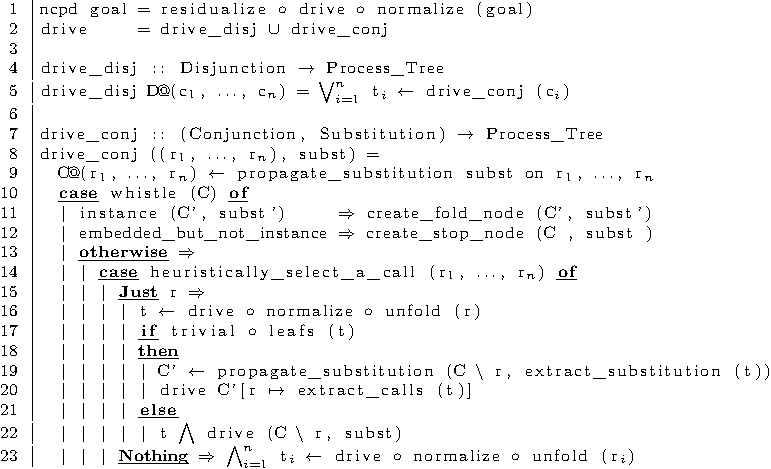
\includegraphics[width=\textwidth]{algo_pseudo-crop.pdf}
  \caption{Conservative partial deduction pseudo code}
  \label{fig:ncpd-pseudo}
\end{figure}

% The very first step of driving a conjunction is to apply a substitution to the variables in relation calls (line 10).

There are several core ideas behind this algorithm.
The first is to select an arbitrary relation to unfold, not necessarily the leftmost which is safe.
The second idea is to use a heuristics which decides if unfolding a relation call can lead to discovery of contradictions between conjuncts which in turn leads to restriction of the answer set at specialization-time (line 14; \code{heuristically\_select\_a\_call} stands for heuristics combination, see section~\ref{sec:heurictic} for details).
If those contradictions are found, then they are exposed by considering the conjunction as a whole and replacing the selected relation call with the result of its unfolding thus \emph{joining} the conjunction back together instead of using \emph{split} as in CPD (lines 15--22).
Joining instead of splitting is why we call our transformer \emph{conservative} partial deduction.
Finally, if the heuristics fails to select a potentially good call, then the conjunction is split into individual calls which are driven in isolation and are never joined (line 23).

When the heuristics selects a call to unfold (line 15), a process tree is constructed for the selected call \emph{in isolation} (line 16).
The leaves of the computed tree are examined.
If all leaves are either computed substitutions or are instances of some relations accompanied with non-empty substitutions, then the leaves are collected and each of them replaces the considered call in the root conjunction (lines 19--20).
If the selected call does not suit the criteria, the results of its unfolding are not propagated onto other relation calls within the conjunction, instead, the next suitable call is selected (line 22).
According to the denotational semantics of \mk it is safe to compute individual conjuncts in any order, thus it is ok to drive any call and then propagate its results onto the other calls.

% Each time we examine a conjunction of calls, we \emph{split} them into separate nodes which are driven independently from each other.
% Among the relation calls we select one which is according to the heuristic is likely to narrow down the answer set \db{(line 15)}.
% If the selected call does not suit the criteria, the results of its unfolding is not propagated onto other relation calls withing the conjunction and the next suitable call is selected \db{(line 22)}.

This process creates branchings whenever a disjunction is examined (lines 4--5).
At each step, we make sure that we do not start driving a conjunction which we have already examined.
To do this, we check if the current conjunction is a renaming of any other configuration in the tree (line 11).
If it is, then we fold the tree by creating a special node which then is residualized into a call to the corresponding relation.

In this approach, we do not generalize in the same fashion as CPD or supercompilation.
Our conjunctions are always split into individual calls and are joined back together only if it is meaningful.
If the need for generalization arises, i.e. homeomorphic embedding of conjunctions~\cite{de1999conjunctive} is detected, then we immediately stop driving this conjunction (line 12).
When residualizing such a conjunction, we just generate a conjunction of calls to the input program before specialization.

% The generalization is used in supercompilation and partial deduction to ensure termination at the same time as some degree of specialization.
% The generalization of two terms is usually a \emph{most-specific generalization}.
% Generalization is used to abstract away some information computed during driving.
% In conjunctive partial deduction generalization is modified to support treating of conjunctions.
% The generalization selects subconjuctions of two conjuncts which are similar (call to the same relation and their arguments have similar shape and distribution).
% For the subconjunctions selected a most-specific generalization is computed.

% In our approach we only do splitting of a conjunction into individual relation calls.
% This makes any program with an accumulating parameter to be a problem.
% Sometimes when there is a need to do a proper generalization, it is in reality just an instance of some other goal within the tree and we can simply create a call there \db{(line 13)}.
% Otherwise we are unable to meaningfully specialize such goal, but we can always just include the initial program in the residual program and call the corresponding relation.


\subsection{Unfolding}

Unfolding in our case is done by substitution of some relation call by its body with simultaneous normalization and computation of unifications.
% To unfold a relation call we do the following steps.
% \db{TODO: the following has alredy mentioned above.}
% First, the formal arguments of a relation are substituted for the actual arguments of the call in the body.
% All fresh variables get instantiated.
% The body is transformed into a canonical form (disjunction of conjunctions of either calls or unifications).
% All unifications are computed.
% Those disjuncts in which unifications fails are removed.
% Other disjuncts take form of a conjunction of relation calls accompanied with a substitution.
The unfolding itself is straightforward; however it is not always clear what to unfold and when to \emph{stop} unfolding.
Unfolding in the context of specialization of functional programming languages, as well as inlining in specialization of imperative languages, is usually considered to be safe from the residual program efficiency point of view.
It may only lead to code explosion or code duplication which is mostly left to a target program compiler optimization or even is out of consideration at all if a specializer is considered as a standalone tool~\cite{jonesbook}.

Unfortunately, this is not the case for the specialization of a relational programming language.
Unlike functional and imperative languages, in logic and relational programming languages unfolding may easily affect the target program's efficiency~\cite{leuschel2002logic}.
Unfolding too much may create extra unifications, which is by itself a costly operation, or even introduce duplicated computations by propagating the results of unfolding onto neighbouring conjuncts.

There is a fine edge between too much unfolding and not enough unfolding.
The former is maybe even worse than the latter.
We believe that the following heuristics provides a reasonable approach to unfolding control.

\subsection{Less Branching Heuristics}
\label{sec:heurictic}

This heuristics is aimed at selecting a relation call within a conjunction which is both safe to unfold and may lead to discovering contradictions within the conjunction.
An unsafe unfolding leads to an uncontrollable increase of the number of relation calls in a conjunction.
It is best to first unfold those relation calls which can be fully computed up to substitutions.

We deem every static (non-recursive) conjunct to be safe because they never lead to growth in the number of conjunctions.
Those calls which unfold deterministically, meaning there is only one disjunct in the unfolded relation, are also considered to be safe.

Those relation calls which are neither static nor deterministic are examined with what we call the \emph{less-branching} heuristics.
It identifies the case when the unfolded relation contains fewer disjuncts than it could possibly have.
This means that we found some contradiction, some computations were gotten rid of, and thus the answer set was restricted, which is desirable when unfolding.
To compute this heuristics we precompute the maximum possible number of disjuncts in each relation and compare this number with the number of disjuncts when unfolding a concrete relation call.
The maximum number of disjuncts is computed by unfolding the body of the relation in which all relation calls were replaced by a unification which always succeeds.

\begin{figure}[!t]
  \centering
  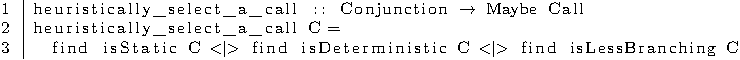
\includegraphics[width=\textwidth]{heuristic-crop.pdf}
  \caption{Heuristics selection pseudocode}
  \label{fig:heu-pseudo}
\end{figure}

%  more complicated case is when there are less disjuncts than there can possibly be.
% This signifies that at least one branch of computations is gotten rid of.

The pseudocode describing our heuristics is shown in Fig.~\ref{fig:heu-pseudo}.
Selecting a good relation call can fail (line 1).
The implementation works such that we first select those relation calls which are static, and only if there are none, we proceed to consider deterministic unfoldings and then we search for those which are less branching.
We believe this heuristics provides a good balance in unfolding.
% The final heuristic selects the first conjunct which suites either of the following cases.
% First we unfold those conjuncts which are static.
% Then --- deterministic.
% Then those which are less branching.
% The last to be unfolded are those calls, which unfold to a substitution with not conjunction.

% \subsection{Residualization}

% Residualization is quite straightforward.
% A branching in the process tree becomes a disjunction.
% A split node becomes a conjunction.
% Computed substitution is residualized as a conjunction of unifications.
% A renaming node is just a call to a relation.
% Relations are created for configurations on which leaf nodes are renamed.

% One other thing is that when some configuration is occurred within the tree which is an instance of a configuration for which a new relation is created, then we just create a call.

\section{Example}

In this section we demonstrate by example how Conservative Partial Deduction works.
The example program is a relational interpreter of propositional formulas under given variable assignments.
The complete code of the example program is provided in Listing~\ref{eval:whole}.

The relation \lstinline{eval$^o$} has three arguments.
The first argument, \lstinline{subst}, is a list of boolean values which plays a role of variable assignments.
The $i$-th value of the substitution is the value of the $i$-th variable.
The second argument, \lstinline{fm}, is a formula with the following abstract syntax.
A formula is either a \emph{variable} represented with a Peano number, a \emph{negation} of a formula, a \emph{conjunction} of two formulas or a \emph{disjunction} of two formulas.
The third argument, \lstinline{res}, is the value of the formula under the given assignment.

The relation \lstinline{eval$^o$} is in canonical normal form: it is a single disjunction which consists of 4 conjunctions of unifications and relation calls, and all its fresh variables are introduced at the top level.
The unification in each conjunction determines the shape of the input formula and binds variables to the corresponding subformulas.
For each of the subformulas, the relation \lstinline{eval$^o$} is called recursively.
Then the results of the evaluation of the subformulas are combined by the corresponding boolean connective to get the result for the input formula.
For example, when the formula is a conjunction of two subformulas \lstinline{x} and \lstinline{y}, the results of their execution \lstinline{v} and \lstinline{w} are combined by the call to the relation \lstinline{and$^o$} to compute the result: \lstinline{and$^o$ v w res}.
If the input formula is a variable, then its value is looked up in the substitution list by means of the relation \lstinline{elem$^o$}.

\begin{figure*}[!t]
  \centering
  \begin{minipage}{0.95\textwidth}
    \begin{lstlisting}[label={eval:whole}, caption={Evaluator of propositional formulas}, captionpos=b, frame=tb]
  let rec eval$^o$ subst fm res = conde [fresh (x y z v w) (
      ( fm === conj x y /\ eval$^o$ st x v /\  eval$^o$ st y w /\  and$^o$ v w res );
      ( fm === disj x y /\ eval$^o$ st x v /\  eval$^o$ st y w /\  or$^o$   v w res );
      ( fm === neg x    /\ eval$^o$ st x v /\  not$^o$ v res );
      ( fm === var v    /\ elem$^o$ subst v res ))]

  let not$^o$  x y = nand$^o$ x x y
  let or$^o$   x y z = nand$^o$ x x xx /\  nand$^o$ y y yy /\ nand$^o$ xx yy z
  let and$^o$ x y z = nand$^o$ x y xy /\   nand$^o$ xy xy z
  let nand$^o$ a b c = conde [
      ( a === ^false /\ b === ^false /\ c === ^true );
      ( a === ^false /\ b === ^true  /\ c === ^true );
      ( a === ^true  /\ b === ^false /\ c === ^true );
      ( a === ^true  /\ b === ^true  /\ c === ^false )]

  let elem$^o$ n subst v = conde [ fresh (h t m) (
    ( n === zero /\ subst === h % t /\ h === v );
    ( n === succ m /\ subst === h % t /\ elem$^o$ m t v ))]


    \end{lstlisting}
  \end{minipage}
\end{figure*}

Consider the goal \lstinline{fresh (s fm) (eval$^o$ s fm ^true)}.
The partially constructed process tree for this goal is presented in Fig.~\ref{fig:evalTree}.
The following notation is used.
Rectangle nodes contain configurations, while diamond nodes correspond to splitting.
Each configuration contains a goal along with a substitution in angle brackets.
To visually differentiate constructors from variables within goals, we made them bold.
For brevity, we only put a fragment of the substitution computed at each step in the corresponding node.
The leaf node which contain only the substitution and no goal in its configuration is a success node.
The call selected to be unfolded is underlined in a conjunction.
Nodes corresponding to failures are not present within the process tree.
Dashed arrows represent renamings.

Conservative partial deduction starts by unfolding the single relation call in this goal once.
Besides introducing fresh variables into the context, unifications in each conjunct are computed into substitutions.
This produces 4 branches, each of which is processed further.

Consider the first branch, in which the input formula \lstinline{fm} is a conjunction of subformulas \lstinline{x} and \lstinline{y}.
First, each of the relation calls within a conjunction is examined to select one of them to unfold.
To do so, we unfold each of them in isolation and use the less branching heuristic.
Since both recursive calls to \lstinline{eval$^o$} are done with three distinct fresh variables, they are not selected.
By unfolding the call to \lstinline{and$^o$} several times, we determine it has less branches than the same relation called on all free and distinct variables (see Fig.~\ref{fig:and}), thus this call is selected to be unfolded.
The result of unfolding the call is a single substitution which associates the variables \lstinline{a} and \lstinline{b} with \lstinline{true}.
By applying the computed substitution to the goal we get a conjunction of two calls to the \lstinline{eval$^o$} relation with the last argument being \lstinline{true}.
This conjunction embeds the root goal, thus we split the conjunction and both calls become leaves which rename the root.
This finishes the processing of the first branch.

Consider the second branch, in which the input formula \lstinline{fm} is a disjunction of subformulas \lstinline{x} and \lstinline{y}.
Similarly to the first branch, the heuristic selects the call to the boolean relation to be unfolded which produces three possible substitutions for variables \lstinline{a} and \lstinline{b}.
The substitutions are propagated into the goals and three branches each of which embeds the root goal is added into the process tree.
Each of the goals is split, then the calls with the last argument being \lstinline{true} rename the root goal.
Then the call \lstinline{eval$^o$ y s false} is processed, which creates 4 branches similar to the branches of the root goal.

The third branch is driven until a call with the last argument being \lstinline{false} is encountered.
Since it renames one of the nodes which is already present in the process tree, we stop exploring this branch and add the back edge.

The last branch, in which the input formula \lstinline{fm} is a variable \lstinline{v}, contain the single call to the relation \lstinline{elem$^o$}.
The unfolding of this call produces two leaves: a success node and a renaming of the parent node.
This finishes the construction of the process tree.

The process tree is then residualized into a specialized version of the \lstinline{eval$^o$} relation.
This program does not contain any calls to boolean connectives.
Neither does the program contain the original, not specialized, relation \lstinline{eval$^o$}.


\begin{figure}[!t]
  \centering
  \begin{minipage}{0.95\textwidth}
    \begin{tikzpicture}[
  processTree]

  \node(0) {\underline{\rel{eval}{\texttt{fm s \textbf{true}}}}};

  \node(00)[below of=0, xshift=-7.5cm, yshift=0.6cm, anchor=north] {
    \rel{eval}{\texttt{x s a}} \conj \\
    \rel{eval}{\texttt{y s b}} \conj \\
    \underline{\rel{and}{\texttt{a b \textbf{true}}}} \\
    \subst{\texttt{fm} $\to$ \texttt{\textbf{conj} x y}}};

  \node(000)[below of=00, anchor=north] {
    \rel{eval}{\texttt{x s \textbf{true}}} \conj \\
    \rel{eval}{\texttt{y s \textbf{true}}} \\
    \subst{\texttt{a} $\to$ \texttt{\textbf{true},} \\ \texttt{b} $\to$ \texttt{\textbf{true}}}};

  \node(0000)[diamond,below of=000, yshift=0.5cm,anchor=north] { \conj };

  \node(00000)[below of=0000, xshift=-1.7cm, yshift=1cm, anchor=north] {
          \rel{eval}{\texttt{x s \textbf{true}}}};
  \node(00001)[below of=0000, xshift=1.7cm, yshift=1cm, anchor=north] {
          \rel{eval}{\texttt{y s \textbf{true}}}};

  \node(01)[below of=0, yshift=0.6cm, anchor=north] {
    \rel{eval}{\texttt{x s a}} \conj \\
    \rel{eval}{\texttt{y s b}} \conj \\
    \underline{\rel{or}{\texttt{a b \textbf{true}}}} \\
    \subst{\texttt{fm} $\to$ \texttt{\textbf{disj} x y}}};

  \node(010)[below of=01, xshift=-3.6cm, anchor=north] {
      \rel{eval}{\texttt{x s \textbf{true}}} \conj \\
      \rel{eval}{\texttt{y s \textbf{true}}} \\
      \subst{\texttt{a} $\to$ \texttt{\textbf{true},} \\ \texttt{b} $\to$ \texttt{\textbf{true}}}};

  \node(0100)[below of=010, anchor=north, draw=none, fill=none, yshift=0.5cm]{...};
  \node(011)[below of=01, anchor=north] {
      \rel{eval}{\texttt{x s \textbf{true}}} \conj \\
      \rel{eval}{\texttt{y s \textbf{false}}} \\
      \subst{\texttt{a} $\to$ \texttt{\textbf{true},} \\ \texttt{b} $\to$ \texttt{\textbf{false}}}};

  \node(0110)[diamond,below of=011, yshift=0.5cm,anchor=north] { \conj };

  \node(01100)[below of=0110, xshift=-1.7cm, yshift=1cm, anchor=north] {
          \rel{eval}{\texttt{x s \textbf{true}}}};
  \node(01101)[below of=0110, xshift=1.7cm, yshift=1cm, anchor=north] {
          \rel{eval}{\texttt{y s \textbf{false}}}};
  \node(011010)[below of=01101, xshift=-1.5cm, yshift=1.5cm, anchor=north, draw=none, fill=none] {...};
  \node(011011)[below of=01101, xshift=-0.5cm, yshift=1.5cm, anchor=north, draw=none, fill=none] {...};
  \node(011012)[below of=01101, xshift=0.5cm,  yshift=1.5cm, anchor=north, draw=none, fill=none] {...};
  \node(011013)[below of=01101, xshift=1.5cm,  yshift=1.5cm, anchor=north, draw=none, fill=none] {...};
  \node(012)[below of=01, xshift=3.7cm, anchor=north] {
      \rel{eval}{\texttt{x s \textbf{false}}} \conj \\
      \rel{eval}{\texttt{y s \textbf{true}}} \\
      \subst{\texttt{a} $\to$ \texttt{\textbf{false},} \\ \texttt{b} $\to$ \texttt{\textbf{true}}}};

  \node(0120)[below of=012, anchor=north, draw=none, fill=none, yshift=0.5cm]{...};


  \node(02)[below of=0, xshift=7.5cm, yshift=0.6cm, anchor=north] {
    \rel{eval}{\texttt{x s a} \conj \\
    \underline{\rel{not}{\texttt{a \textbf{true}}}} \\
    \subst{\texttt{fm} $\to$ \texttt{\textbf{neg} x}}}};

  \node(020)[below of=02,yshift=-0.23cm, anchor=north] {
    \rel{eval}{\texttt{x s \textbf{false}}} \\
    \subst{\texttt{a} $\to$ \texttt{\textbf{false}}}};

  \node(03)[below of=0, xshift=11.5cm, yshift=0.6cm, anchor=north] {
    \rel{elem}{\texttt{x s \textbf{true}}} \\
    \subst{\texttt{fm} $\to$ \texttt{\textbf{var} v}}
  };

  \node(030)[below of=03, xshift=-1cm, anchor=north, yshift=-0.5cm]{
    \subst{\texttt{s} $\to$ \texttt{h\%t}, \\ \texttt{x} $\to$ \texttt{\textbf{zero}} \\ \texttt{h} $\to$ \texttt{\textbf{true}}}
  };
  \node(031)[below of=03, xshift=2cm, anchor=north, yshift=-0.5cm]{
    \rel{elem}{\texttt{y t \textbf{true}}} \\
    \subst{\texttt{s} $\to$ \texttt{h\%t}, \\ \texttt{x} $\to$ \texttt{\textbf{succ} y}}};


  \draw [->] (0.south west) to (00.north east);
  \draw [->] (0) to (01);
  \draw [->] (0) to (02.north west);
  \draw [->] (0.south east) to (03.north west);
  \draw [->] (00) to (000);
  \draw [->] (000) to (0000);
  \draw [->] (0000) to (00000);
  \draw [->] (0000) to (00001);
  \draw [->] (01) to (010);
  \draw [->] (01) to (011);
  \draw [->] (01) to (012);
  \draw [->] (010) to (0100);
  \draw [->] (011) to (0110);
  \draw [->] (0110) to (01100);
  \draw [->] (0110) to (01101);
  \draw [->] (01101) to (011010);
  \draw [->] (01101) to (011011);
  \draw [->] (01101) to (011012);
  \draw [->] (01101) to (011013);
  \draw [->] (012) to (0120);
  \draw [->] (02) to (020);
  \draw [->] (03) to (030);
  \draw [->] (03) to (031);

  \draw [dashed,<-] ($(0.south west)+(0.1,0)$) .. controls +(-5,-2.5) and +(-4,0) .. (01100.west);
  \draw [dashed,->] (00000.north west) to [out=90,in=180] ($(0.west)$);
  \draw [dashed,->] (00001) to [out=90,in=-135] ($(0.west)+(0,-0.1)$);

  \draw[dashed,->] (020.south) to [out=-90,in=0] (01101.east);
  \draw[dashed,->] (031.north east) to [out=90,in=0] (03.south east);

\end{tikzpicture}
  \end{minipage}
  \caption{Partially constructed process tree for the relation eval$^o$.}
  \label{fig:evalTree}
\end{figure}

\begin{figure*}[!t]
  \centering
  \begin{minipage}{0.95\textwidth}
    \begin{lstlisting}[label={eval:whole}, caption={Specialized evaluator of propositional formulas}, captionpos=b, frame=tb]
  let rec eval$^o_{true}$ subst fm = conde [fresh (x y z v w) (
      ( fm === conj x y /\ eval$^o_{true}$ st x /\  eval$^o_{true}$ st y );
      ( fm === disj x y /\ (conde [
          ( eval$^o_{true}$ st x /\    eval$^o_{true}$ st y );
          ( eval$^o_{true}$ st x /\    eval$^o_{false}$ st y );
          ( eval$^o_{false}$ st x /\    eval$^o_{true}$ st y );
      ]);
      ( fm === neg x /\ eval$^o_{false}$ st x v );
      ( fm === var v /\ elem$^o_{true}$ subst v ))]

  let rec eval$^o_{false}$ subst fm = conde [fresh (x y z v w) (
      ( fm === conj x y /\ (conde [
          ( eval$^o_{false}$ st x /\    eval$^o_{false}$ st y );
          ( eval$^o_{true}$ st x /\    eval$^o_{false}$ st y );
          ( eval$^o_{false}$ st x /\    eval$^o_{true}$ st y );
      ]);
      ( fm === disj x y /\ eval$^o_{true}$ st x /\  eval$^o_{true}$ st y );
      ( fm === neg x /\ eval$^o_{true}$ st x v );
      ( fm === var v /\ elem$^o_{false}$ subst v ))]

  let elem$^o_{true}$ n subst = conde [ fresh (h t m) (
      ( n === zero /\ subst === true % t );
      ( n === succ m /\ subst === h % t /\ elem$^o_{true}$ m t ))]

  let elem$^o_{false}$ n subst = conde [ fresh (h t m) (
      ( n === zero /\ subst === false % t );
      ( n === succ m /\ subst === h % t /\ elem$^o_{false}$ m t ))]


    \end{lstlisting}
  \end{minipage}
\end{figure*}
\section{Evaluation}

We implemented the conservative partial deduction for \mk and compared it with the \ecce partial deduction system.
\ecce is designed for \pro programming language and cannot be directly applied for programs, written in \mk.
To be able to compare our approach with \ecce, we converted each input program first to the pure subset of \pro, then specialized it with \ecce, and then we converted the result back to \mk.
The conversion to \pro is a simple syntactic conversion. In the conversion from \pro to \mk, for each Horn clause a conjunction is generated in which unifications are placed before any relation call.

We chose two problems for our study: evaluation of a subset of propositional formulas and typechecking for a simple language.
The problems illustrate the approach of using relational interpreters to solve search problems~\cite{lozov2019relational}.
For both these problems we considered several possible implementations in \mk which highlight different aspects relevant in specialization.

The \lstinline{eval$^o$} relation implements an evaluator of a subset of propositional formulas.
We consider four different implementations of this relation to explore how the way program is implemented can affect the quality of specialization.
Depending on the implementation, \ecce generates programs of varying performance, while the execution times of the programs generated by our approach are similar.

The \lstinline{typecheck$^o$} relation implements a typechecker for a tiny expression language.
We consider two different implementations of this relation: one written by hand and the other generated from the functional program.
We demonstrate how much these implementations differ in terms of performance before and after specialization.

In this study we measured the execution time for the sample queries, averaging them over multiple runs.
We also measured the number of unifications done in search of each individual answer.
All examples of \mk relations in this paper are written in \oc\footnote{\oc: statically typed \mk embedding in \ocaml. The repository of the project: \url{https://github.com/JetBrains-Research/OCanren}}.
The queries were run on a laptop running Ubuntu 18.04 with quad core Intel Core i5 2.30GHz CPU and 8 GB of RAM.

The tables and graphs use the following denotations.
\emph{Original} represents the execution time of a program before any transformations were applied; \emph{ECCE}~--- of the program specialized by \ecce with default conjunctive control setting; \emph{ConsPD}~--- of the program specialized by our approach.

\subsection{Evaluator of Logic Formulas}

The relation \lstinline{eval$^o$} describes an evaluation of a propositional formula under given variable assignments.
The relation has three arguments. The first argument is a list of boolean values which plays a role of variable assignments.
The $i$-th value of the substitution is the value of the $i$-th variable.
The second argument is a formula with the following abstract syntax.
A formula is either a \emph{variable} represented with a Peano number, a \emph{negation} of a formula, a \emph{conjunction} of two formulas or a \emph{disjunction} of two formulas.
The third argument is the value of the formula under the given assignment.

We specialize the \lstinline{eval$^o$} relation to synthesize formulas which evaluate to \lstinline{^true}.
To do so, we run the specializer for the goal with the last argument fixed to \lstinline{^true}, while the first two arguments remain free variables.
Depending on the way the \lstinline{eval$^o$} is implemented, different specializers generate significantly different residual programs.

\subsubsection{The Order of Relation Calls}

One possible implementation of the evaluator is presented in Listing~\ref{eval:last}.
Here relation \lstinline{elem$^o$ subst v res} unifies \lstinline{res} with the value of the variable \lstinline{v} in the list \lstinline{subst}.
The relations \lstinline{and$^o$}, \lstinline{or$^o$}, and \lstinline{not$^o$} encode corresponding boolean connectives.

\begin{figure*}[!t]
  \centering
  \begin{minipage}{0.95\textwidth}
    \begin{lstlisting}[label={eval:last}, caption={Evaluator of formulas with boolean operation last}, captionpos=b, frame=tb]
  let rec eval$^o$ subst fm res = conde [fresh (x y z v w) (
      (fm === conj x y /\ eval$^o$ st x v /\  eval$^o$ st y w /\  and$^o$ v w res);
      (fm === disj x y /\ eval$^o$ st x v /\  eval$^o$ st y w /\  or$^o$   v w res);
      (fm === neg x    /\ eval$^o$ st x v /\  not$^o$ v res));
      (fm === var v    /\ elem$^o$ subst v res)]
    \end{lstlisting}
  \end{minipage}
  \begin{minipage}{0.95\textwidth}
    \begin{lstlisting}[label={eval:fst}, caption={Evaluator of formulas with boolean operation second}, captionpos=b, frame=tb]
  let rec eval$^o$ subst fm res = conde [fresh (x y z v w) (
      (fm === conj x y /\ and$^o$ v w res /\  eval$^o$ st x v /\  eval$^o$ st y w);
      (fm === disj x y /\ or$^o$   v w res /\ eval$^o$ st x v /\  eval$^o$ st y w);
      (fm === neg x    /\ not$^o$ v res   /\ eval$^o$ st x v);
      (fm === var v    /\ elem$^o$ subst v res))]
    \end{lstlisting}
  \end{minipage}
\end{figure*}

Note, the calls to boolean relations \lstinline{and$^o$}, \lstinline{or$^o$}, and \lstinline{not$^o$} are placed last within each conjunction.
This poses a challenge for the CPD-based specializers such as \ecce.
Conjunctive partial deduction unfolds relation calls from left to right, so when specializing this relation for running backwards (i.e. considering the goal \lstinline{eval$^o$ subst fm ^true}), it fails to propagate the direction data onto recursive calls of \lstinline{eval$^o$}.
Knowing that \lstinline{res} is \lstinline{^true}, we can conclude that in the call \lstinline{and$^o$ v w res} variables \lstinline{v} and \lstinline{w} have to be \lstinline{^true} as well.
There are three possible options for these variables in the call \lstinline{or$^o$ v w res} and one for the call \lstinline{not$^o$}.
These variables are used in recursive calls of \lstinline{eval$^o$} and thus restrict the result of driving.
CPD fails to recognize this, and thus unfolds recursive calls of \lstinline{eval$^o$} applied to fresh variables.
It leads to over-unfolding, large residual programs and poor performance.

The conservative partial deduction first unfolds those calls which are selected according to the heuristics.
Since exploring the implementations of boolean connectives makes more sense, they are unfolded before recursive calls of \lstinline{eval$^o$}.
The way conservative partial deduction treats this program is the same as it treats the other implementation in which boolean connectives
are moved to the left, as shown in Listing~\ref{eval:fst}.
This program is easier for \ecce to specialize which demonstrates how unequal the behaviour of CPD for similar programs is.

\subsubsection{Unfolding of Complex Relations}

Depending on the way a relation is implemented, it may take a different number of driving steps to reach the point when any useful information is derived through its unfolding.
Partial deduction tries to unfold every relation call unless it is unsafe, but not all relation calls serve to restrict the search space and thus should be unfolded.
In the implementation of \lstinline{eval$^o$} boolean connectives can effectively restrict variables within the conjunctions and should be unfolded until they do.
But depending on the way they are implemented, the different number of driving steps should be performed for that.
The simplest way to implement these relations is by mimicking a truth tables as demonstrated by the implementation of \lstinline{not$^o$} in Listing~\ref{not:table}.
It is enough to unfold such relation calls once to derive useful information about variables.

\begin{figure*}[!t]
  \centering
  \begin{minipage}{0.5\textwidth}
    \begin{lstlisting}[label={not:table}, caption={Implementation of boolean \lstinline{not} as a table}, captionpos=b, frame=tb]
  let not$^o$ x y = conde [
     (x === ^true /\ y === ^false;
      x === ^false /\ y === ^true)]
    \end{lstlisting}
  \end{minipage}
  \begin{minipage}{0.8\textwidth}
    \begin{lstlisting}[label={not:nando}, caption={Implementation of boolean operation via \lstinline{nand}}, captionpos=b, frame=tb]
  let not$^o$   x y = nand$^o$ x x y
  let or$^o$   x y z = nand$^o$ x x xx /\  nand$^o$ y y yy /\ nand$^o$ xx yy z
  let and$^o$ x y z = nand$^o$ x y xy /\   nand$^o$ xy xy z
  let nand$^o$ a b c = conde [
    ( a === ^false /\ b === ^false /\ c === ^true );
    ( a === ^false /\ b === ^true  /\ c === ^true );
    ( a === ^true  /\ b === ^false /\ c === ^true );
    ( a === ^true  /\ b === ^true  /\ c === ^false)]
    \end{lstlisting}
  \end{minipage}
\end{figure*}

The other way to implement boolean connectives is to express them using a single basic boolean relation such as \lstinline{nand$^o$} which is, in turn, has a table-based
implementation (see Listing~\ref{not:nando}). It will take several sequential unfoldings to derive that variables \lstinline{v} and \lstinline{w} should
be \lstinline{^true} when considering a call \lstinline{and$^o$ v w ^true} implemented via a basic relation.
Conservative partial deduction drives the selected call until it derives useful substitutions for the variables involved while CPD with deterministic unfolding may fail to do so.


\subsubsection{Evaluation Results}

In our study we considered 4 implementations of \lstinline{eval$^o$} summed up in the table~\ref{tbl:eval}. They differ in the way the boolean connectives are implemented (see column \emph{Implementation}) and whether they are placed before or after the recursive calls to \lstinline{eval$^o$} (see column \emph{Placement}).
These four implementations are very different from the  standpoint of \ecce.

\begin{table}[!h]
    \centering
    \begin{tabular}{c||c||c}
                      & Implementation & Placement \\ \hline\hline
    \emph{FirstPlain} & table-based    & before \\ \hline
    \emph{LastPlain}  & table-based    & after  \\ \hline
    \emph{FirstNando} & via nand$^o$   & before \\ \hline
    \emph{LastNando}  & via nand$^o$   & after  \\
    \end{tabular}

  \caption{Different implementations of eval$^o$}
  \label{tbl:eval}
\end{table}

We measured the time necessary to generate $1000$ formulas over two variables which evaluate to \lstinline{^true} (averaged over 10 runs).
The results are presented in Fig.~\ref{fig:eval}.

\begin{figure}[!t]
  \centering
  \begin{subfigure}[c]{0.35\textwidth}
    \centering
    \begin{tabular}{e{1cm}||c|c|c}
               & Original & \ecce & ConsPD \\ \hline\hline
      \emph{FirstPlain} & 1.59s & 1.61s & 0.92s \\ \hline
      \emph{FirstNando} & 1.43s & 2.24s & 0.96s \\ \hline
      \emph{LastPlain}  & 0.98s & 1.43s & 0.97s \\ \hline
      \emph{LastNando}  & 1.09s & 1.54s & 0.91s
    \end{tabular}
  \end{subfigure}
  \hfill
  \begin{subfigure}[c]{0.58\textwidth}
    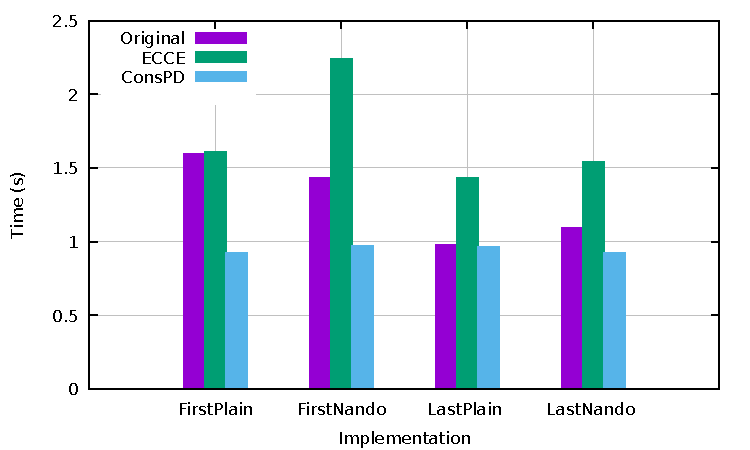
\includegraphics[width=\textwidth]{data/propEval/prop.pdf}
  \end{subfigure}
  \caption{Execution time of evalo}
  \label{fig:eval}
\end{figure}

Conservative partial deduction generates  programs with comparable performance for all four implementations, while the quality of \ecce specialization differs significantly.
\ecce worsens performance for every implementation as compared to the original program.
ConsPD do not worsen performance for any implementation.
Its effect is most significant for the implementations in which the boolean connectives are placed first within conjunctions.

\subsubsection{The Order of Answers}

It is important to note that different implementations of the same \mk relation produce answers in different orders.
Nevertheless, since \mk search is complete, all answers will be found eventually.
Unfortunately, it is not guaranteed that the first 1000 formulas generated with different implementations of \lstinline{eval$^o$} will be the same.
For example, $983$ formulas are the same among the first $1000$ formulas generated by the Original \emph{FirstPlain} relation and the same relation after the ConsPD transformation.
At the same time, only $405$ formulas are the same between the Original and \ecce \emph{LastNando} relations.

The reason why implementations differ so much in the order of the answers stems from the canonical search strategy employed in \mk.
Most \mk implementations employ \emph{interleaving} search~\cite{10.1145/1090189.1086390} which is left-biased.
It means that the leftmost disjunct in a relation is being executed longer than the disjunct on the right.
This property is not local which makes it very hard to estimate the performance of a given relation.

In practice it means that if a specializer reorders disjuncts, then the performance of relations after specialization may be unpredictable.
For example, by putting the disjuncts of the \lstinline{eval$^o$} relation in the opposite order, one produces a relation which runs much faster than the original, but it generates completely different formulas at the same time.
Most of the first 1000 formulas in this case are multiple negations of a variable, while the original relation produces more diverse set of answers.
Computing a negation of a formula only takes one recursive \lstinline{eval$^o$} call thus finding such answers is faster than conjunctions and disjunctions.
Meanwhile, the formulas generated by the reordered relation are less diverse and may be of less interest.

Although neither \ecce nor ConsPD reorder disjuncts, they remove disjuncts which cannot succeed.
Thus they influence the order of answers and performance of relations.
We believe that, in general, it is not possible to guarantee the same order of answers after specialization.
Exploring how different specializations influence the execution order is a fascinating direction for future research.


\subsection{Typechecker-Term Generator}

This relation implements a typechecker for a tiny expression language.
Being executed in the backward direction it serves as a generator of terms of the given type.
The abstract syntax of the language is presented below.
The variables are represented with de Bruijn indices, thus let-binding does not specify which variable is being bound.

\[\begin{array}{lllll}
  type \ term = &\ BConst \ of \ Bool &| \ IConst \ of \ Int &| \ Var \ of \ Int & \\
  & | \ term + term &| \ term * term &| \ term = term &| \ term < term \\
  &| \ \underline{let} \ term \ \underline{in} \ term
  &\multicolumn{2}{l}{| \ \underline{if} \ term \ \underline{then} \ term \ \underline{else} \ term} &
\end{array}\]

The typing rules are straightforward and are presented below.
Boolean and integer constants have the corresponding types regardless of the environment.
Only terms of type integer can be summed up, multiplied or compared by less-than operator.
Any terms of the same type can be checked for equality.
Addition and multiplication of two terms of suitable types have integer type, while comparisons have boolean type.
If-then-else expression typechecks only if its condition is of type boolean, while both then- and else-branches have the same type.
An environment $\Gamma$ is an ordered list, in which the $i$-th element is the type of the variable with the $i$-th de Bruijn index.
To typecheck a let-binding, first, the term being bound is typechecked and is added in the beginning of the environment $\Gamma$, and then the body is typechecked in the context of the new environment.
Typechecking a variable with the index $i$ boils down to getting an $i$-th element of the list.

\begin{table}[!h]
  \setlength{\tabcolsep}{0.4cm}
  \centering
  \begin{tabular}{c c c}
    \infer[]{\Gamma \vdash IConst \ i : Int}{} &
    \infer[]{\Gamma \vdash BConst \ b : Bool}{}  &
    \infer[\Gamma \lbrack v \rbrack \equiv \tau]{\Gamma \vdash Var \ v : \tau}{} \vspace{0.5cm}
    \\
    \infer[]{\Gamma \vdash t + s : Int}{\Gamma \vdash t : Int, \Gamma \vdash  s : Int}  \vspace{0.5cm} &
    \infer[]{\Gamma \vdash t = s : Bool}{\Gamma \vdash t : \tau, \Gamma \vdash  s : \tau} &
    \infer[]{\Gamma \vdash \underline{let} \ v \ b : \tau}{\Gamma \vdash v : \tau_v, \ (\tau_v :: \Gamma) \vdash b : \tau}
      \\

      \infer[]{\Gamma \vdash t * s : Int}{\Gamma \vdash t : Int, \Gamma \vdash  s : Int}  &
    \infer[]{\Gamma \vdash t < s : Bool}{\Gamma \vdash t : Int, \Gamma \vdash  s : Int} \vspace{0.5cm} &
      \infer[]{\Gamma \vdash \underline{if} \ c \ \underline{then} \ t \ \underline{else} \ s : \tau}{\Gamma \vdash c : Bool, \Gamma \vdash t : \tau, \Gamma \vdash s : \tau}
  \end{tabular}
\end{table}


We compared two implementations of these typing rules.
The first one is obtained by unnesting of a functional program as described in~\cite{lozov2019relational} (\emph{Generated}).
It is worth noting that the unnesting introduces a lot of redundancy in form of extra unifications and thus creates programs which are very inefficient.
Thus we contrast this implementation with the program hand-written in \oc (\emph{Hand-written}).
Each implementation has been specialized with ConsPD and \ecce.
We measured the time needed to generate 1000 closed terms of type integer (see Fig.~\ref{tbl:type}).


\begin{figure}[!h]
  \begin{subfigure}[c]{0.55\textwidth}
    \centering
    \begin{tabular}{c||c|c|c}
                          & Original & \ecce & ConsPD  \\ \hline\hline
      \emph{Hand-written} & 0.92s    & 0.22s & 0.34s   \\ \hline
      \emph{Generated}    & 11.46s   & 0.38s & 0.29s
      \end{tabular}
  \end{subfigure}
  \hfill
  \begin{subfigure}[c]{0.45\textwidth}
    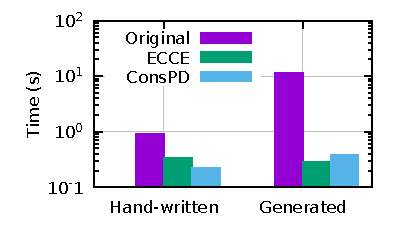
\includegraphics[width=\textwidth]{data/lTypecheck/ltypelog.pdf}
  \end{subfigure}
  \caption{Execution  time of generating 1000 closed terms of type Integer}
  \label{tbl:type}
\end{figure}

As expected, the generated program is far slower than the hand-written.
The principal difference between these two implementations is that the generated program contains a certain redundancy introduced by unnesting.
For example, typechecking of the sum of two terms in the hand-written implementation consists of a single conjunction (see Listing~\ref{type:hand}) while the generated program is far more complicated and also uses a special relation \lstinline{typeEq$^o$} to compare types (see Listing~\ref{type:gen}).

\begin{figure*}[!h]
  \centering
    \begin{lstlisting}[label={type:hand}, caption={A fragment of hand-written typechecker}, captionpos=b, frame=tb]
  let rec typecheck$^o$ gamma term res = conde [
    ...
    fresh (x y) ((term === x + y /\
       typecheck$^o$ gamma x ^(Some Integer) /\
       typecheck$^o$ gamma y ^(Some Integer) /\
       res === ^(Some Integer)));
    ...]
    \end{lstlisting}
\end{figure*}


\begin{figure*}[!t]
  \centering
    \begin{lstlisting}[label={type:gen}, caption={A fragment of generated typechecker}, captionpos=b, frame=tb]
let rec typecheck$^o$ gamma term res = conde [
  ...
  fresh (x y t1 t2) ((term === x + y /\
    conde [
      typecheck$^o$ gamma x ^None       /\ res === ^None;
      typecheck$^o$ gamma x ^(Some t1) /\
        typecheck$^o$ gamma y ^None     /\ res === ^None;
      typecheck$^o$ gamma x ^(Some t1) /\  typecheck$^o$ gamma y ^(Some t2) /\
        typeEq$^o$ t1 Integer ^true     /\ typeEq$^o$ t2 Integer ^true /\
        res === ^(Some Integer);
    ])
  ...]
    \end{lstlisting}
\end{figure*}

Most of the redundancy of the generated program is removed by specialization with respect to the known type of the term.
This is why both implementations have comparable speed after specialization.
\ecce shows bigger speedup for the hand-written program than ConsPD and vice versa for the generated implementation.
We believe that this difference can be explained by too much unfolding.
\ecce performs a lot of excessive unfolding for the generated program and only barely changes the hand-written program.
At the same time ConsPD specializes both implementations to comparable programs performing average amount of unfolding.
This shows that the heuristics we presented gives more stable, although not the best, results.

% У заключения нет номера главы
\clearpage

\section*{Заключение}
В ходе данной работы получены следующие результаты. 
\begin{itemize}
  \item Изучена предметная область: методы обработки встроенных языков и алгоритм обобщённого синтаксического анализа RNGLR.
  \item Разработан алгоритм синтаксического анализа динамически формируемых выражений, поддерживающий работу с произвольными входными графами.
  \item Доказана корректность алгоритма:
  \begin{itemize}
    \item алгоритм завершит работу для любых входных данных;
          %для любой входной детерминированной контекстно-свободной грамматики и 
          %произвольного входного графа алгоритм завершит свою работу;
    \item для любой цепочки из входного множества, выводимой в эталонной грамматике G, в SPPF содержится её дерево вывода в G; при этом никакие другие деревья не содержатся в SPPF.
          %для любой цепочки, которую может породить автомат (которая содержится 
          %в регулярном множестве), выводимой в рассматриваемой грамматике G, в 
          %SPPF содержится её дерево вывода в G, при этом не содержится никаких 
          %других деревьев.
  \end{itemize}
  \item Выполнена реализация алгоритма на языке программирования F\# в рамках исследовательского проекта YaccConstructor.
  \item Проведена апробация: регрессионное тестирование, тестирование производительности и тестирование на реальных данных.
  \item Исходный код проекта YaccConstructor можно найти на сайте \url{https://github.com/YaccConstructor/YaccConstructor}, автор принимал участие под учётной записью kajigor.
\end{itemize}

В дальнейшем планируется изменить алгоритм таким образом, чтобы помимо 
построения леса разбора всех корректных выражений осуществлялся бы также поиск ошибочных выражений и сообщение о них. Также необходимо произвести теоретическую оценку сложности алгоритма. Предложенный алгоритм планируется внедрить в инструмент по реинжинирингу информационных систем.  

\nocite{*}
\bibliographystyle{eptcs}
\bibliography{bibl.bib}

\newpage

\section*{Appendix}

We thank the reviewers for their thoughtful feedback.


\subsection*{Review 1}

The paper considers the optimisation of miniKanren relational programs using some form of (conjunctive) partial evaluation. In particular, the authors propose a novel approach, called conservative partial deduction, and reports on an experimental evaluation that compares the results obtained with ECCE (an online partial evaluator for Prolog based on conjunctive partial deduction) and the authors' tool. The results are very promising and show the advantages of the new approach.

All in all, the paper contains interesting ideas and I recommend it to be accepted for VPT 2021.

% \emph{Thank you for the kind review.}

Detailed comments for authors:

\begin{itemize}
  \item In order for the paper to be as self-complete as possible, I'd suggest to add a brief introduction to miniKanren (syntax, informal semantics, a couple of examples) at the beginning of the paper.

  \emph{Added. See subsection \ref{mkIntro}.}

  \item There are already some works that considered non-leftmost unfolding during partial evaluation, e.g.,

  \begin{itemize}
    \item  E. Albert, G. Puebla, J.P. Gallagher: Non-leftmost Unfolding in Partial Evaluation of Logic Programs with Impure Predicates. LOPSTR 2005: 115-132
    \item M. Leuschel, G. Vidal: Fast offline partial evaluation of logic programs. Inf. Comput. 235: 70-97 (2014)
  \end{itemize}

  \emph{Thank you for bringing these to our attention. }
  \todo{Check: non-leftmost unfolding of what? What's the motivation?}

  \item As for the effectiveness of partial evaluation, you can check this one

  \begin{itemize}
    \item G. Vidal: Cost-Augmented Partial Evaluation of Functional Logic Programs. High. Order Symb. Comput. 17(1-2): 7-46 (2004)
  \end{itemize}

  where the effectiveness of partial evaluation is estimated, and this one

  \begin{itemize}
    \item G. Vidal: Trace Analysis for Predicting the Effectiveness of Partial Evaluation. ICLP 2008: 790-794
  \end{itemize}

  which aims at predicting the effectiveness achieved by partial evaluation
  (though it's just a preliminary approach).

  \emph{Thank you! These papers do provide a nice way to estimate how efficient a transformation is and we will likely employ these ideas in future versions of our specializer, although this would likely require some tweaking for the interleaving semantics of \mk. }

  \item The formalisation of conservative partial deduction using pseudocode is nice, but a more formal approach (as in [3]) might be useful to prove a number of properties. You could consider that as future work.

  \emph{We agree that our approach will benefit from a more formal description and will consider it as future work.}

  \item{In Sect. 3.1, you mention that unfolding too much might introduce extra unifications or duplicate computations. I think that this is not possible as long as partial evaluation considers a fixed left-to-right unfolding strategy at PE time. This is actually a problem when considering non-leftmost unfolding strategies at PE time.}

  \emph{Section 5.1.1 of the paper~\cite{de1999conjunctive} states that non-determinate unfolding may add unifications regardless of wether the unfolding strategy is left-to-right or not. Of course, in pure \pro the effect of using unfolding strategies which are not left-to-right is more pronounced. Nevertheless, interleaving semantics of \mk complicates everything even further.}

  \item Another unfolding strategy that might be related to your heuristics
  is presented in

  \begin{itemize}
    \item G. Vidal: A Hybrid Approach to Conjunctive Partial Evaluation of Logic
    Programs. LOPSTR 2010: 200-214
  \end{itemize}

  where the notion of ``strongly regular logic programs'' is introduced in order to characterise the predicates whose unfolding cannot produce infinitely growing conjunctions at PE time.

  \todo{Check: It seems that there are not that many evaluators which are strongly regular logic programs.}

  \item {The experimental evaluation is certainly promising. Nevertheless,
  it would be great if you could put the implemented tool publicly available,
  including the source code of the considered benchmarks so that the readers
  can replicate the experiments.}

  \emph{The tool is available on github: \url{https://github.com/kajigor/uKanren_transformations/}, the experiments, currently not very well structured, are also on github in a different repository: \url{https://github.com/kajigor/mk-transformers-bench}}
\end{itemize}


\subsection*{Review 2}

This paper looks at partial deduction for the relational programming language  MINIKANREN. The execution of programs in MINIKANREN differs from that in Prolog in that the subgoals of a conjunction or disjunction can be reordered. This creates many more degrees of freedom in the way a program can be executed, and also in the optimisations that can be performed.

The paper looks at issues faced by conjunctive partial deduction of MINIKANREN and describes a new approach to partial deduction for relational languages called conservative partial deduction. The main issue with conjunctive partial deduction of MINIKANREN is the unfolding strategy. For Prolog, this is usally done by deterministic unfolding where all atoms except one are only unfolded if it matches with at most one clause head. One atom, usually the leftmost one, can be unfolded non-deterministically. However, this can add many new relation calls to a conjunction. Although this works well for Prolog, it does not work so well for MINIKANREN as it does not match its order of evaluation and can result in large less efficient programs.

\emph{Thank you for the detailed and accurate summary. This shows that we were able to communicate our intent well.}

The solution proposed to this problem in this paper is called conservative partial deduction, which is inspired by both partial deduction and supercompilation. One aim is to create a speialization algorithm that is simpler than conjunctive partial deduction, but I am not sure this has been achieved as it still seems quite complex.

\emph{We agree that our approach is not the simplest, but we still strive towards this goal.}

The conservative aspect of the algorithm is in the unfolding of relation calls. This involves deciding if unfolding a relation call can lead to discovery of contradictions between conjuncts which in turn leads to restriction of the answer set at specialization-time. It is unclear how exactly this is preferrable to unfolding any other relation call.

\emph{The core idea behind this approach is in removing (at specialization-time) those computations which will definitely fail at run-time. To do so we examine which calls within a conjunction interact in such a way as to lead to failures (one may say, the calls contradict each other), and if there are such calls, we process as a whole conjunction rather than splitting and driving them separately, loosing the information about contradictions by doing so.}

It might actually add many new relation calls to a conjunction and result in large less efficient programs. The result of the unfolding is joined back into the conjunction rather than being split as is done in conjunctive partial deduction. It also just stops on encountering an embedding rather than trying to generalise and further transform.

\emph{This decision was made in pursuit of reducing the algorithm's complexity. There is no reason not to do generalization of goals which do not require splitting.}

The algorithm does not take advantage of the fact that subgoals in the language can be reordered, so it appears to miss out on many further opportunities for optimisation.

\emph{On the contrary, whenever the algorithm decides that some call within a conjunction may lead to contradiction, it unfolds the call and replaces it with the result of unfolding. This, at specialization-time, changes the order in which the calls are executed (see how boolean connectives are processed in different implementations of the} \lstinline{eval$^o$} \emph{relation). The residualized program will have the calls (or rather the result of unfolding of the calls) in roughly the same order, which was our intention from the very beginning.}

The evaluation of the proposed technique is rather poor, with only variations of two test programs being evaluated. For the evaluator of logic formulas, the variations are on the way the boolean connectives are implemented, and whether these connectives are placed before or after the recursive call. For the type checker, the variations are on whether it was implemented by hand or  automatically generated from a corresponding functional program. This is not enough to conclude whether the transformation works well in practice.

\emph{We agree this evaluation is not enough, and we are working on the better set of benchmarks. These programs were chosen to demonstrate typical issues which occur in developping efficient relational interpreters. Our goal in selecting them was to provide non-trivial examples which are illustrative and can be easily comprehended by the reader.}

The transformed programs do all perform better than the original program, but ECCE does perform better than the described transformation for one program variation. The order of the answers produced by transformed programs can also be different to that of the original program, which I see as very problematic as the transformation is changing the behaviour of the program.

\emph{The search in \mk is complete, thus all possible answers will be found, given enough time. This is why the \mk community does not focus on the order in which answers are found. The denotational semantics of a \mk program is a set of relations on the free variables of a goal rather that the list of answers in any particular order. See~\cite{rozplokhas2020certified} for the proof of the equivalence of the denotational and operational semantics of \mk.}

Although the paper is well written, the contributions it makes to the area are minimal. It does not seem appropriate to apply conjunctive partial deduction to transform MINIKANREN programs, as conjunctive partial deduction follows the evaluation strategy of logic languages such as Prolog rather than that of relational languages such as MINIKANREN. It would seem to be more appropriate to devise a new transformation that follows the search strategy used by the MINIKANREN implementation.

\emph{We believe that using a well-established framework for specialization of a language related to \mk is the most reasonable first step. If it had worked right away, we would have just applied CPD and moved on to the next challenge. Alas, it did not work as well as we hopped, thus we proceeded to developping a different transformation.}

For the correctness of the transformation, it should be proved that the transformation does not change the order of answers produced for the program.

\emph{According to the denotational semantics, the order of answers does not matter. Once we establish the best specialization method for \mk, we will prove its correctness with respect to the denotational semantics of \mk.}

A more thorough evaluation of the described technique is also required. I am therefore on the fence as to whether to accept this paper or not.

\emph{We agree with the need for better evaluation.}

Detailed Comments
=================

Section 1, second last para: This opens a yet another possibility $\to$ This opens yet another possibility

Section 2, para 2: is so-called process tree $\to$ is a so-called process tree

Section 2, para 2: Of course, process tree $\to$ Of course, the process tree

Section 2, para 2: signalls $\to$ signals

Section 2, para 3: the efficiency of residual program $\to$ the efficiency of a residual program

Section 2, para 3: yielding standalone compilation more powerful $\to$ making standalone compilation more powerful

Section 2, final para: empitical $\to$ empirical

Section 3, para 5: use a heuristics which decides $\to$  use a heuristic which decides

Section 3, para 5: if the heuristics fails to select $\to$ if the heuristic fails to select

\emph{Thank you spending you time on finding and correcting all these mistakes. English is our second language and we are happy every time someone points out a missing article or incorrect spelling, since it gives us a chance to improve.}


Section 3, final para: only if it is meaningful - what is meant by ``meaningful''?

\emph{Here it was used as a more formal synonym for ``if it makes sense''.}

Section 3.1, para 2: Unlike functional and imperative languages, in logic and relational programming languages unfolding
may easily affect the target program’s efficiency - actually unfolding in functional and imperative languages can also
affect the program's efficiency if paramters are non-linear.

\emph{We agree that unfolding may decrease the performance of programs with non-linear arguments for functional and imperative languages. }

\todo{Add something about non-linearity being everywhere in \mk programs, and point out that using non-linear arguments is crucial.}

Section 3.2, Figure 2: this figure is not really necessary and does not add very much

Section 3.2, para 3: the less-branching heuristics $\to$ the less-branching heuristic

Section 4, para 4: generated from the functional program - you have not really said what this functional program is

\emph{We meant the straightforward implementation of the interpreter in a functional language which was then translated into \mk by means of relational conversion, according to the approach described in~\cite{lozov2019relational}.}

Section 4.1.1, para 2: direction data - it is not clear what is meant by this

\emph{We specialize a \mk goal in which some of the arguments are known statically. Which arguments are known and which are free variables determines the ``direction'' in which relation call is executed. See the second and the third paragraphs of the seciton~\ref{intro}. }

Section 4.1.2, para 1: mimicking a truth tables $\to$ mimicking a truth table

Section 4.2, para 3: in form of extra unifications $\to$ in the form of extra unifications

Section 5, para 1: which uses a heuristics $\to$ which uses a heuristic

Section 5, para 2: with regrads to $\to$ with regards to

Section 5, para 3: were improved better $\to$ were improved more

\emph{We thank you again for the detailed feedback. We value your work.}
\subsection*{Review 3}
The paper has been revised, but my opinion of the quality and significance of the paper has not been improved.  Generally, the points that were mentioned in my first review were not satisfactorily addressed.

The goal of running relational programs backwards is definitely a challenging and interesting problem.  However, this experiment does not advance our understanding of the problem and its possible solutions.

The proposed "novel approach" (less branching heuristic) is to select goals for unfolding that are either deterministic (so that unfolding cannot increase the search space), or result in some pruning of the search space by discovering failures.  These are relevant heuristics, but are not so different from existing strategies for unfolding during partial evaluation of logic programs, which are also related to well known search heuristics such as the "first-fail" and "forward-checking" principles. The analysis and evaluation of the heuristic is quite limited.

The comparison with ECCE is inadequate and nothing significant can be concluded from it.  Firstly, the existing facilities in ECCE are not exploited (only default settings are tried) and there is no analysis of the reasons why ECCE does not produce the desired result (perhaps resulting in trying some other ECCE options).  Secondly, the Prolog programs presented to ECCE are translated from MiniKanren using a naive DNF-based translation, which can introduce inefficiencies that ECCE is not designed to handle.  The approach consists of taking a program P1 in MiniKanren, translating it to program P2 in Prolog, which is possibly far less efficient than P1 due to duplication of goals and extra backtracking introduced by DNF translation, then apply ECCE leading to P3, which may still contains the search overhead of P2.  P1 is also specialised using the MiniKanren partial evaluator, yielding P4. Then P3 and P4 are compared, running both in MiniKanren. There are so many factors to consider that could affect performance, yet this paper ignores them. The response to the first review mentions some potential benefits of the DNF form for detecting failures, but this is not convincing and not discussed in the paper, though it could possibly be important. Finally, very few programs are tested, and running times are small, reducing the significance of the evaluation.

My recommendation would be to develop a specialiser for MiniKanren, and perform significant tests on a wide variety of MiniKanren programs.  Where relevant, experience from ECCE and other Prolog partial evaluators can be transferred to MiniKanren, but a direct comparison with ECCE is not meaningful.

However, in its present form, I cannot recommend acceptance.

Some detailed comments
======================

page 2, lines 1-6 (under fig 1).  This paragraph is confused and misleading.  The model semantics of Prolog is independent of the order of body goals.  This is exploited by Prolog transformation tools, even without changing the operational behaviour of Prolog.  E.g. See ref [1] which you cite, and ECCE itself. The impression is given that this is a special new feature of MiniKanren.

\emph{The paragraph is rewritten to better convey what we meant. Unlike \pro, operational semantics of \mk is complete. It is also equivalent to the denotational semantics of \mk. This means that no new answers will be found and no existing answers will be lost when \mk program is transformed by switching around subgoals. Tranforming \mk program may only affect the termination of the \mk interpreter when it is asked to find more answers than there exists.}

page 3, line 1.  typo substuting

  Section 2.2.  Relational interpreters are interesting, but from the point of view of specialisation they do not present any different problems than other relations.  If so, please explain how.

line -2.  "Search problems are notoriously complicated."  This is a meaningless statement.  In what sense are they "more complex than verification", given that verification is undecidable, and that even in finite cases, the verification of a forall property can require the whole search space to be traversed.

\emph{It is usually harder for a human programmer to come up with an algorithm for the search program, as compared to the corresponding verification problem.}

\subsection*{Review 4}
This revised version of the paper has been improved as compared with the version accepted in the first round of reviewing, but still there are flaws to be corrected.

The authors hide carefully what is a contribution of the paper, forcing the reader to look for the contribution over all details presented in the whole paper. There is still no transparent list of authors' contributions in the introduction marked clearly with the word "Contributions:". That is exactly the main problem of the presentation, mentioned by the reviewers in the first round of reviewing.
Nevertheless this reviewer was able to find something in the revised version, what is maybe one of contribution of the paper. So I suppose the following might be pretend to be a novelty contributed by the authors.

Heads of clauses in programs written in logical or relational languages include quite often multiple occurrences of variables to be unified. As a rule, the values of such variables are used for specifying the conditions of exits from recursions. Unification against such a clause takes a time that is not uniformly bounded over size of input data. Thus the runtime complexity, by default, assumed by the unfolding operation becomes inadequate. The unfolding may generate too many clauses of a residual predicate definition, along which clause-wise backtracking is very time expensive. The authors try to control such a situation and propose a heuristic being responsible for balancing between enough many of unfolding steps and enough little of the syntactic branchings in the residual programs.

In general terms not using by the authors, the heuristic can be described, for example, as follows.
Given a configuration including a number of function or relation calls, which may be reordered in such a way that the configuration's result does not depend on the order chosen for computing the calls. As a rule, the unfolding and whole specialization process will lead to better results if the first call to be specialized is a call that can be most specialized (i.e. more efficiently, meaning the result) as compared to the specialization results of the other calls in the configuration.

Another flaw: the authors use actively the supercompilation terminology, although do often that in incorrect ways, but no reference to Valentin Turchin, who is the founder of the supercompilation method, is included.  A number of references to original Turchin's works have to be given in the paper.

The introduction consists mainly of modified cites taken from other authors and misunderstood by these paper' authors.

A list of additional concrete remarks, suggestions, and typos can be found below.


1 Introduction
1) Page 1
You write: "The search employed in MINIKANREN is complete which means that every answer will be found, although it may take a long time."

It may non-terminate rather than only take a long time, if a relation encoded with a program has infinite domain that have to be found, i.e., actually, a component of the corresponding Cartesian product.

\emph{If a \mk relation has a finite number of answers $n$ and a user asks for $m \leq n$ answers, then \mk interpreter will find all the answers eventually. If a user asks for $m > n$ answers, then, after finding all $n$ answers, \mk interpreter can either terminate or not terminate --- this depends on the \mk program. If there are infinitely many answers, and a user asks for $m$ answers, then $m$ answers will be found eventually. If a user asks for all the answers and there are infinitely many answers, then non-termination is unavoidable, but \mk interpreter will not get stuck exploring some failing brunch forever, it will still produce answers.}

2) Page 1
You write: "An earlier paper [22] has shown that conjunctive partial deduction [5] can sometimes improve the performance of MINIKANREN programs."

Actually it was shown much earlier in the context of whole logical programming.

3) Page 2
The introduction should include a paragraph starting with the following words: Our contributions: …
Where all the subjects, that you deem your contributions, should be briefly and explicitly listed with using theirs meaning rather than only names.
For example, use of  "the conservative partial deduction" in the list, without an additional brief explanation, is a bad idea.


3 Related Work
4) Page 4
You write: "The heart of supercompilation-based techniques is driving - a symbolic execution of a program through all possible execution paths. The result of driving is a possibly infinite process tree where nodes correspond to configurations which represent computation _state_."

    a) Unfortunately, the authors do not understand the essence of one of the basic concepts of supercompilation, namely the driving.
    b) Typo:  state $\rightarrow$ states

5) Page 4
You write: "Each path in the tree corresponds to some concrete program execution."

That is wrong. For example, the unfolding of any unconditional one step program results in the only parameterized path corresponding to all concrete executions.

6) Page 4
You write: "When the tree is constructed, the resulting, or residual, program can be extracted from the process tree by the process called residualization."

 This contradicts a sentence written a couple lines above (as well as the next your sentence): "The result of driving is a possibly infinite process tree …".  Actually, the residual program is extracted from the corresponding finite residual graph.


7) Page 5
You write: "The specialization is done in two levels of control: the local control determines the shape of the residual programs, while the global control ensures that every relation which can be called in the residual program is defined. The leaves of local control trees become nodes of the global control tree. CPD analyses these nodes at the global level and runs local control for all those which are new."

The first sentence is misleading while at the first glance the third one shows the fact that the authors unawares of the huge amount literature about the question discussed, but it is only partly true.


8) Page 5
You write: "At the local level, CPD examines a conjunction of atoms by considering each atom one-by-one from left to right. An atom is unfolded if it is deemed safe, i.e. a whistle based on homeomorphic embedding does not signal for the atom.
When an atom is unfolded, a clause whose head can be unified with the atom is found, and a new node is added into the tree where the atom in the conjunction is replaced with the body of that clause."

  The first statement is wrong once again. It contradicts the second one, since the unfolding can recurrently increase the number of atoms in a conjunction of a configuration.
  The home homeomorphic embedding should control the size of the whole configuration rather than any atom standing alone.
  The authors go on pretending that they are unaware of the tupling program transformation method aiming at rearranging the structure of configurations in the process tree and opening opportunities for improving runtime complexity of the residual program as compared with an input program to be transformed. Please, study also a more fundamental concept of the function circuit widely used in the computation complexity theory and having direct relation to the tupling method. The last two our sentences also are directly related to your last paragraph in this section.

\emph{Default CPD uses homeomorphic embedding on the local control level to select an atom to unfold. It does not unfold an atom which has an ancestor in the local control tree which is embedded into the atom (see page 252, definition 3.8 in~\cite{de1999conjunctive}). At the global control level, an extension of the homeomorphic embedding for conjunctions is applied to the whole configuration. }



4 Conservative Partial Deduction
9) Page 6, The algorithm pseudocode is shown in Fig. 2.
You write: "A driving process (along with generalization and folding) creates a process tree …"

 Immediately after the very first folding action the process tree become a process graph rather than a tree. That is the main aim of the folding. Too many such a "tree process" term are encountered in your paper and misleading the reader.  Thus I am forced to think the authors do not understand the background being considered.

\emph{In our implementation, process graphs are represented as trees, since trees can be straightforwardly represented with an ADT and are easier to use. Backedges thus are not actually edges: when folding a special leaf node is added into the tree, this node has its ancestors' configuration stored in it. It complicates residualization, while making everything else easier. This implementation design decision clearly seeped into the text. We fixed the terminology. }

10) Page 6, The algorithm pseudocode is shown in Fig. 2.
You write: "The nodes of the process tree include a configuration which describes the state of program evaluation at some point."

Typos: The nodes of the process tree include  … $\rightarrow$ Given a node of the process tree, it includes a configuration …

11) Page 6, The algorithm pseudocode is shown in Fig. 2.
You write: "The substitution computed at each step is also stored in the tree node, although it is not included in the configuration. This means that only the goal, and not the substitution, is passed into the whistle to determine potential non-termination."

(a) How I see you mean here the narrowing substitution. Actually I doubt strongly that your partial deduction tool being developed terminates without generalizing the narrowing substitutions, since a relation domain may be infinite and as a consequence the corresponding narrowing substitutions may indefinitely grow in their sizes. This problem should be clarified.

\emph{\mk programs execute to a stream of substitutions as per the operational semantics of \mk. While driving, we compute unifications into substitutions, and store them alongside conjunctions in nodes. We always apply corresponding substitutions to conjunctions, thus there is no need to generalize them. }

(b) I do not think that it is a good idea to use the vulgar meaningless term "whistle", though a number of authors use such a "term" in the same context.

12) Page 7, The algorithm pseudocode is shown in Fig. 2.
You write: "In this approach, we do not generalize in the same fashion as CPD or supercompilation. This decision was motivated by keeping the complexity of the approach to the minimum. Our conjunctions are always split into individual calls and are joined back together only if it is meaningful, for example, leads to contradictions. If the need for generalization arises, i.e. homeomorphic embedding of conjunctions [5] is detected, then we immediately stop driving this conjunction (line 12). When residualizing such a conjunction, we just generate a conjunction of calls to the input program before specialization."

Is the explanation above the main contribution done in the paper? If it is true then you have to evidently write it in the introduction, using the word "contribution".
Actually I do not think that such a decision is a novel one, since it is trivial and was certainly tried by a huge amount of researchers in the branch of program specialization and refused since no interesting transformations may be expected using such a kind of  "generalization".

4.1 Unfolding
13) Page 8
You write: "Unfolding too much may create extra unifications, which is by itself a costly operation, or even introduce duplicated computations by propagating the results of unfolding onto neighbouring conjuncts."

In the first round review I wrote "Actually none can reason on any efficiency without fixing an efficiency model. And so on … (See my first review.)"
Your remark above is exactly about this notion. Please read once again my first review. Actually similar problems are encountered in the context of specialization of functional programs.
I do not believe that your remark and corresponding approach are original. As a rule such a problem is taken into account with additional program transformation tools that are invoked only after the main stage of specialization.


4.2 Less Branching Heuristic
14) Page 8
You write: "Selecting a good relation call can fail (line 1)."

Actually the first line contains only the signature of the function. That should be corrected.

\emph{The signature states that the result is \code{Maybe Call} which expresses that the result is optional. Clarified it in the text.}

5 Example
15) Page 9, Listing 2
The meaning of the percent sign should be either commented or replaced with the standard colon sign widely used for the infix constructor standing for Cons.

16) Page 10, Figure 4:
You write: "Partially constructed process tree for the relation evalo."

process tree $\rightarrow$ process graph

17) Page 10, Figure 4:
You write: "Since both recursive calls to evalo are done with three distinct fresh variables, they are not selected according to the less branching heuristic."

This statement means nothing. In general it cannot be the reason of the delay of the evalo calls, since unification of the calls against clauses' heads might be uniform, i.e. it might be done without any narrowing some of the fresh variables. The sentence should be rewritten.

\emph{\mk does not unify calls against clauses' head, since there are no clauses in \mk programs. The heuristic selects those atoms which have strictly less branches in their unfolding than it's possible. There cannot be more branches than when a call with all arguments fresh and distinct variables is considered.}


18) Page 11, Listing 3: Specialized evaluator of propositional formulas
The presented example is clear, but too very simple. Let it be. None of possible problems that you try to overcome has been demonstrated with a corresponding specialization example.


19) Page 12
You write: "It is worth noting that the result produced by the Conservative Partial Deduction is not ideal. For example, in the definition of the evalo_true, when the input formula fm is a disjunction of subformulas x and y, the recursive call evalo_true s x is done twice in two disjuncts. The ideal version of the relation evalo_true should contain this recursive call only once. However, ideally, y should not be evaluted at all, since the value of the formula fm does not depend on it. It is unclear if and how this kind of transformation can be done automatically."

It is not a problem, meaning this example. The corresponding redundant call should be cleaned by a post processing.
But, in general, it is certainly that the problem is undecidable. It is quite natural. Isn't it?


6 Evaluation
6.1.1 The Order of Relation Calls
20) Page 13
You write: "The conservative partial deduction first unfolds those calls which are selected according to the heuristic. Since exploring the implementations of boolean connectives makes more sense, they are unfolded before the recursive calls of evalo. The way conservative partial deduction treats this program is the same as it treats the other implementation in which boolean connectives are moved to the left, as shown in Listing 5. This program is easier for ECCE to specialize which demonstrates how unequal the behaviour of CPD for similar programs is."

It is not news. Any researcher having a real practical experience in developing any program specialization tool is aware of the problem and the heuristic described and tested by you. You formulate the heuristic, usually named a strategy, in specific MiniKanren terms. That confuses the reader, obscures the essence of the problem and heuristic considered. Actually the heuristic can be described in general terms revealing its essence,
for example, as follows.

Given a configuration including a number of function or relation calls which may be reordered in such a way that the configuration's result does not depend on the order chosen for computing the calls. As a rule, the unfolding and whole specialization process will lead to better results if the first call to be specialized is a call that can be most specialized (i.e. more efficiently, meaning the result) as compared to the specialization results of the other calls in the configuration.

It is rather a thesis (a principle) than a heuristic.

6.2 Typechecker-Term Generator
21) Page 16
You write: "An environment G is an ordered list, …"

By definition, any list is ordered. Any "unordered list" is named a set.


6.3 Discussion: Tupling and Deforestation
22) Page 18
A couple of references to the tupling methods should be given. The tupling method originates from A. Pettorossi and was improved by W.N. Chin.


7 Conclusion
23) Page 19
You write: "We conclude that there is still not one good technique which definitively speeds up every relational program."

If one mean not only trivial program transformations then such a technique does not exist at all, since the corresponding problem is undecidable. It is our life.

Acknowledgements
24) Page 19
Typo: … fruitful discussiona … $\rightarrow$ … fruitful discussions …


References
25) Page 20
You write: "[4] William E Byrd, Eric Holk \& Daniel P Friedman (2012): …"

There are a number of such a kind of typos in the list of the references (the dot signs are absent after the seconds capitalized letters):
William E Byrd $\rightarrow$ William E. Byrd
Daniel P Friedman $\rightarrow$ Daniel P. Friedman

26) Page 20
You write: "[7] Jason Hemann Daniel P Friedman: … "

Typo: the comma sign is absent:
Hemann $\rightarrow$ Hemann,

27) Page 20
You write:
" [7] Jason Hemann Daniel P Friedman: mKanren: A Minimal Functional Core for Relational Programming.
  [8] John P Gallagher (1993): Tutorial on specialisation of logic programs. In: Proceedings of the 1993 ACM SIGPLAN symposium on Partial evaluation and semantics-based program manipulation, pp. 88-98, doi:10.1145/154630.154640."

All the references in the reference list have to be represented in the common fashion required by the EPTCS team. The two references cited above are written in two different fashions.


28) Page 20
The paper uses actively the supercompilation terminology, although does often that in incorrect ways, but no reference to V.F. Turchin, who is the founder of the supercompilation method, is included.
A number of references to original Turchin's works have to be given and cited in the paper.


\subsection*{Review 5}

Post-review:

The paper has been improved significantly. I enjoyed reading the examples in detail. The points about the evaluation are well taken. I'm looking forward to the follow-up work.

Minor point:

num/sum in Listing 1 are barely readable (but in the text below they read fine).

\todo{\emph{It was a weird artefact of lstlising, fixed. }}



\end{document}
